\documentclass{article}
\usepackage{ctex}
\usepackage{cite}
\usepackage{graphicx}
\usepackage{amsmath}

\usepackage[left=2.5cm, right=2.5cm, top=2.8cm, bottom=2.8cm]{geometry}

\usepackage{algorithm}  
\usepackage{algorithmicx}  
\usepackage{algpseudocode} 

\usepackage{tikz}
\usetikzlibrary{positioning, shapes.geometric}

\begin{document}

\thispagestyle{empty}

% \begin{algorithm}[h]
%     \caption{BA算法}
%     \begin{algorithmic}[1] %每行显示行号  
%         \Require 散点数据集$ \mathbf{P} = \{ x_{c}, y_{c}, z_{c}, v_{c} \} $
%         \Ensure 控制栅格$ \Phi = \{ \phi_{ijk} \} $
%         \For{all $ i,j $}
%         \State $ \delta_{ijk} = 0 $ and $ \omega_{ijk} = 0 $
%         \EndFor
%         \For{each point $ \left( x_{c}, y_{c}, z_{c}, v_{c} \right) $ in $ \mathbf{P} $}
%         \State let $ i = \left[ x_{c} \right] - 1 $ and $ j = \left[ y_{c} \right] - 1 $ and $ k = \left[ z_{c} \right] - 1 $
%         \State let $ r = x_{c} - \left[ x_{c} \right] $ and $ s = y_{c} - \left[ y_{c} \right] $ and $ t = z_{c} - \left[ z_{c} \right] $
%         \State compute $ w_{ijk} $'s and $ \sum_{d=0}^{3}\sum_{e=0}^{3}\sum_{g=0}^{3}w_{deg}^{2} $
%         \For{$ i,j,k = 0,1,2,3 $}
%         \State compute $ \phi_{ijk} $ with Formula 2-5
%         \State add $ w_{ijk}^{2}\phi_{ijk} $ to $ \delta_{\left( a+i \right)\left( b+j \right)\left( c+k \right)} $
%         \State add $ w_{ijk}^{2} $ to $ \omega_{\left( a+i \right)\left( b+j \right)\left( c+k \right)} $
%         \EndFor
%         \EndFor
%         \For{all $ i,j $}
%         \If { $ \omega_{ijk} \neq 0 $ }
%         \State compute $ \phi_{ijk} = \delta_{ijk} / \omega_{ijk} $
%         \Else { let $ \phi_{ijk} = 0 $ }
%         \EndIf
%         \EndFor
%     \end{algorithmic}
% \end{algorithm}

% \newline
% \begin{figure}
%     \centering
%     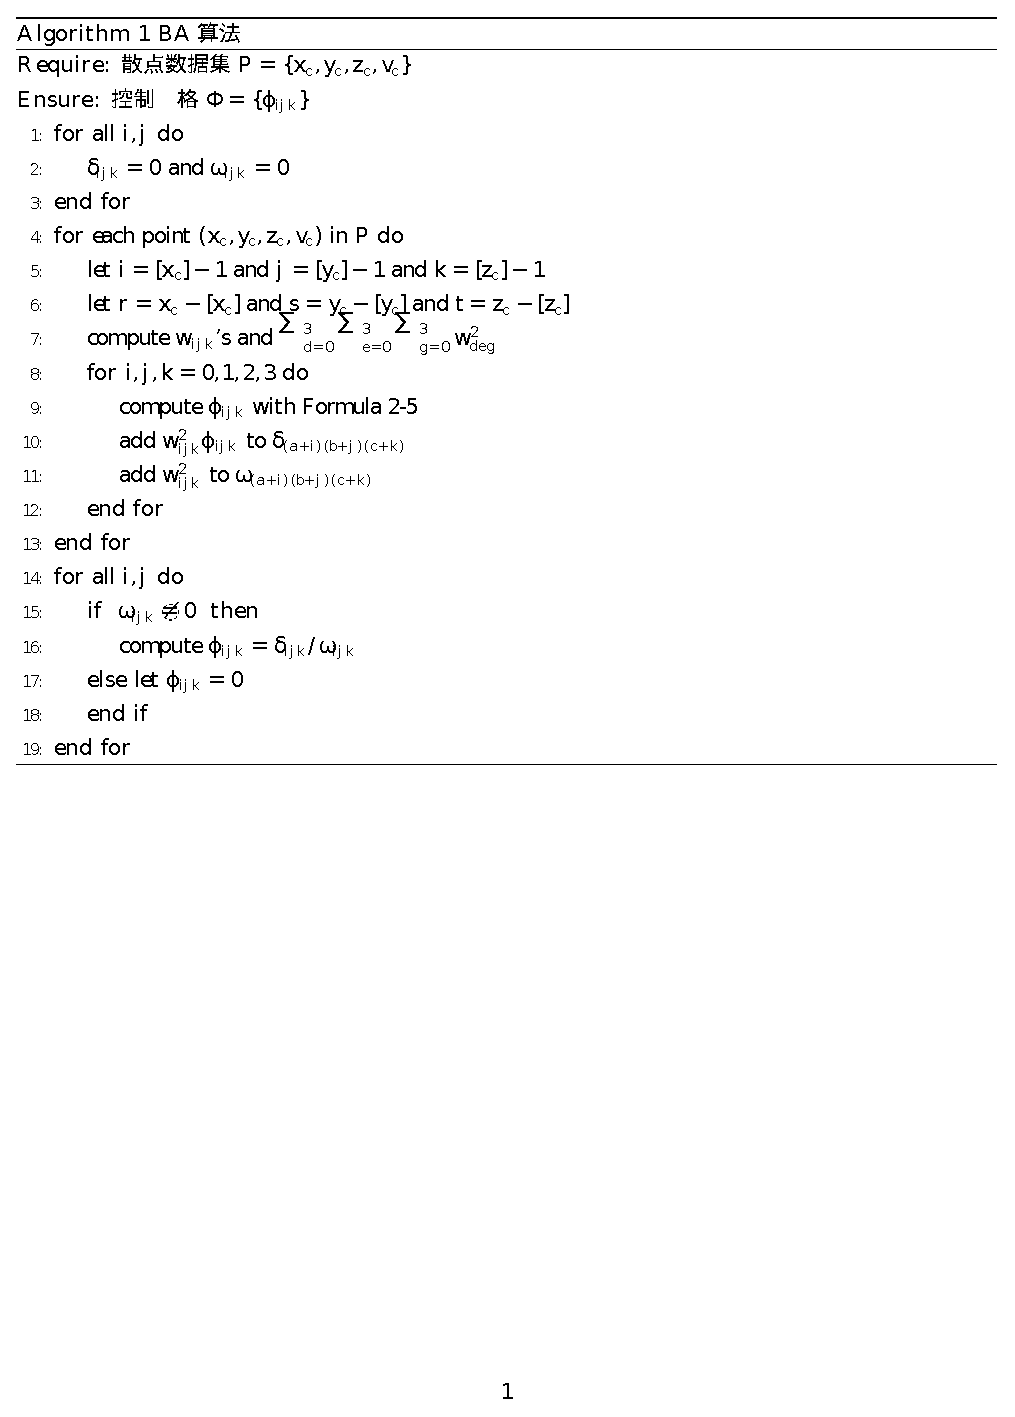
\includegraphics[width=0.9\textwidth]{main.eps}
% \end{figure}

% \begin{algorithm}
%     \caption{MBA算法}
%     \begin{algorithmic}[1] %每行显示行号  
%         \Require 散点数据集$ \mathbf{P} = \{ x_{c}, y_{c}, z_{c}, v_{c} \} $
%         \Ensure 多层控制栅格$ \Phi_{0},\Phi_{1},\cdots,\Phi_{h} $
%         \State let $ k = 0 $
%         \While{$ k \leq h $}
%         \State let $ \mathbf{P_{k}} = \{ \left( x_{c}, y_{c}, z_{c}, \bigtriangleup^{k}v_{c} \right) \} $
%         \State compute $ \Phi_{k} $ from $ \mathbf{P_{k}} $ by BA algorithm
%         \State compute $ \bigtriangleup^{k+1}v_{c} = \bigtriangleup^{k}v_{c} - f_{k}\left( x_{c}, y_{c}, z_{c} \right) $ for each data point
%         \State let $ k = k+1 $
%         \EndWhile
%     \end{algorithmic}
% \end{algorithm}

% \begin{algorithm}
%     \caption{MBA优化算法}
%     \begin{algorithmic}[1] %每行显示行号  
%         \Require 散点数据集$ \mathbf{P} = \{ x_{c}, y_{c}, z_{c}, v_{c} \} $
%         \Ensure 控制栅格$ \Psi $
%         \State let $ \Phi = \Phi_{0} $
%         \State let $ \Psi^{'} = 0 $
%         \While{$ \Phi \neq \Phi_{h} $}
%         \State compute $ \Phi $ from $ \mathbf{P} $ by the BA algorithm
%         \State compute $ \mathbf{P} = \mathbf{P} - F\left( \Phi \right) $
%         \State compute $ \Psi = \Psi^{'} + \Phi $
%         \State let $ \Phi_{k} = \Phi_{k+1} $
%         \State refine $ \Psi $ into $ \Psi^{'} $ whereby $ F\left( \Psi^{'} \right) = F\left( \Psi \right) $ and $ | \Psi^{'} | = | \Phi | $
%         \EndWhile
%     \end{algorithmic}
% \end{algorithm}

\begin{figure}
    \centering
    \begin{tikzpicture}[node distance=10pt]
        \node[draw, rounded corners]                        (start)   {开始};
        \node[draw, below=of start]                         (step 1)  {导入数据};
        \node[draw, below=of step 1]                        (step 2)  {计算Kriging插值重构辐射场};
        \node[draw, below=of step 2]                        (step 3)  {计算Spline插值重构辐射场};
        \node[draw, below=of step 3]                        (step 4)  {计算两个重构辐射场的偏差};
        \node[draw, diamond, aspect=6, below=of step 4]     (choice)  {偏差值是否大于设定值};
        \node[draw, right=20pt of choice]                   (step x)  {添加测量数据};
        \node[draw, below=20pt of choice]                   (step 5)  {绘制空间辐射场};
        \node[draw, below=of step 5]                        (step 6)  {计算整体偏差};
        \node[draw, rounded corners, below=of step 6]       (end)     {结束};

        \draw[->] (start)  -- (step 1);
        \draw[->] (step 1) -- (step 2);
        \draw[->] (step 2) -- (step 3);
        \draw[->] (step 3) -- (step 4);
        \draw[->] (step 4) -- (choice);
        \draw[->] (choice) -- (step 5);
        \draw[->] (choice) -- node[left]  {否} (step 5);
        \draw[->] (choice) -- node[above] {是}  (step x);
        \draw[->] (step 5) -- (step 6);
        \draw[->] (step x) -- (step x|-step 1) -> (step 1);
        \draw[->] (step 6) -- (end);
    \end{tikzpicture}
    % \caption{辐射场重构算法程序框图}
    % \label{辐射场重构算法程序框图}
\end{figure}

\end{document}